\documentclass[aspectratio=169,a4paper,10pt]{beamer}
%%% Local Variables:
%%% mode: latex
%%% TeX-master: t
%%% End:


%% PACKAGES POUR BEAMER

\usetheme{metropolis}
\usepackage[utf8]{inputenc}
\usepackage[T1]{fontenc}
\usepackage[french]{babel}
\usepackage{appendixnumberbeamer}
\usepackage{booktabs}
\usepackage[scale=2]{ccicons}
\usepackage{xspace}
\newcommand{\themename}{\textbf{\textsc{metropolis}}\xspace}
%%
\usepackage{bookmark}
\usepackage{tikz}
\usepackage{wrapfig}
\usepackage{multicol}
\usepackage{subfig}
\usepackage{color} % package des couleurs
\usepackage{xcolor}
\usepackage{graphicx}
\usepackage{pgfplots}
\usetikzlibrary{plotmarks}
\usepackage{pst-all}
\usepackage{lmodern}
\usepackage{multimedia}
\usepackage{media9}
\usepackage{cancel}

%% style des pages
\usepackage{fancyhdr}
%\pagestyle{fancy}

\usepackage{multimedia}
\usepackage{media9}
\usepackage[framemethod=tikz]{mdframed}

%% maths
\DeclareMathOperator{\e}{e}
\usepackage{mathtools}
\usepackage{amsfonts}
\usepackage{amsmath}
\usepackage{amssymb}
\usepackage{hyperref}
\usepackage{esvect}
\usepackage{upgreek}
\usetikzlibrary{shadows}
\usetikzlibrary{backgrounds}
\usepackage{transparent}



%% environnements


\definecolor{definitionf}{RGB}{220,252,220}
\definecolor{definitionl}{RGB}{39,123,69}
\definecolor{definitiono}{RGB}{72,148,101}


%%%%%%%%%% DEFINITION
\newmdenv[tikzsetting={fill=definitionf}, linewidth=2pt, linecolor=definitionl, outerlinewidth=0pt, innertopmargin=5pt, innerbottommargin=5pt, innerleftmargin=5pt, innerrightmargin=5pt, leftmargin=0pt]{defi}

\newmdenv[ tikzsetting={drop shadow={ shadow xshift=1ex, shadow yshift=-1em, fill=definitiono, opacity=1, every shadow } }, outerlinewidth=2pt, outerlinecolor=white, linecolor=white, innertopmargin=0pt, innerbottommargin=0pt, innerleftmargin=0pt, innerrightmargin=0pt]{ombredef}



%%%%%%%%%% THEOREME
\definecolor{theof}{RGB}{255,216,218}
\definecolor{theol}{RGB}{160,0,4}
\definecolor{theoo}{RGB}{221,65,100}


\newmdenv[tikzsetting={fill=theof}, linewidth=2pt, linecolor=theol, outerlinewidth=0pt, innertopmargin=5pt, innerbottommargin=5pt, innerleftmargin=5pt, innerrightmargin=5pt, leftmargin=0pt]{theo}

\newmdenv[ tikzsetting={drop shadow={ shadow xshift=1ex, shadow yshift=-0.5em, fill=theoo, opacity=1, every shadow } }, outerlinewidth=2pt, outerlinecolor=white, linecolor=white, innertopmargin=0pt, innerbottommargin=0pt, innerleftmargin=0pt, innerrightmargin=0pt]{ombretheo}

%%%%%%%%%%%%%%%%%%%%%%%%%%%%%%%%%%%%%%%%%%%%%%%%%%%%%%%%%%%%%%%%%%%%%%%%%%%%%%%%
%% Logo

%% Insert the logo figures here
\titlegraphic{%
  \centering
  %\hspace{3cm}
  \vspace{-.5cm}
    
\includegraphics[scale=.3]{figures/ESPCI.jpg}\hspace{3cm}
    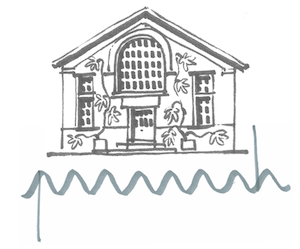
\includegraphics[scale=.5]{figures/PMMH.png}\hspace{2cm}
    %
\includegraphics[scale=.13]{figures/anr-logo.png}\hfill
}
%%%%%%%%%%%%%%%%%%%%%%%%%%%%%%%%%%%%%%%%%%%%%%%%%%%%%%%%%%%%%%%%%%%%%%%%%%%%%%%%

%%%%%%%%%%%%%%%%%%%%%%%%%%%%%%%%%%%%%%%%%%%%%%%%%%%%%%%%%%%%%%%%%%%%%%%%%%%%%%%%
%% Title page

\makeatletter
\setbeamertemplate{title page}{
  \begin{minipage}[t][\paperheight]{\textwidth}
    \ifx\inserttitle\@empty\else\usebeamertemplate*{title}\fi
    \ifx\insertsubtitle\@empty\else\usebeamertemplate*{subtitle}\fi
    \usebeamertemplate*{title separator}
    \begin{center}
    \ifx\beamer@shortauthor\@empty\else\usebeamertemplate*{author}\fi
    \ifx\insertinstitute\@empty\else\usebeamertemplate*{institute}\fi
    \ifx\insertdate\@empty\else\usebeamertemplate*{date}\fi
    
    \end{center}
    \vspace{.3cm}
    \ifx\inserttitlegraphic\@empty\else\inserttitlegraphic\fi
    %\vspace*{.2cm}
  \end{minipage}
}

%% FOOTLINE
\setbeamertemplate{footline}{
\leavevmode%

\hbox{\hspace*{-0.06cm}
\begin{beamercolorbox}[wd=.2\paperwidth,ht=2.25ex,dp=1ex,center]{author in head/foot}%
%\usebeamerfont{author in head/foot}\insertshortauthor\hfill
\insertframenumber{} / \inserttotalframenumber\hspace*{2ex}
\end{beamercolorbox}%

\begin{beamercolorbox}[wd=.6\paperwidth,ht=2.25ex,dp=1ex,center]{section in head/foot}%
\usebeamerfont{section in head/foot}%\insertshorttitle
\end{beamercolorbox}%

\begin{beamercolorbox}[wd=.2\paperwidth,ht=2.25ex,dp=1ex,right]{section in head/foot}%
%\usebeamerfont{section in head/foot}\hspace*{2em}
\usebeamerfont{section in head/foot}
%\insertframenumber{} / \inserttotalframenumber\hspace*{2ex}
\end{beamercolorbox}}%

\vskip0pt%
}
\makeatother

%%%%%%%%%%%%%%%%%%%%%%%%%%%%%%%%%%%%%%%%%%%%%%%%%%%%%%%%%%%%%%%%%%%%%%%%%%%%%%%%



\usepackage{soul}
\usepackage{fancybox}
\renewcommand{\thefootnote}{}
\def\checkmark{\tikz\fill[scale=0.6, definitionl](0,.35) -- (.25,0) -- (1,.7) -- (.25,.15) -- cycle;}
\newsavebox\MBox
\newcommand\Cline[2][red]{{\sbox\MBox{$#2$}%
  \rlap{\usebox\MBox}\color{#1}\rule[-1.\dp\MBox]{\wd\MBox}{0.5pt}}}


\graphicspath{{figures/Introduction/}{figures/Vorticite/}{figures/Bateaux/}{figures/annexes/}}
\title{\vspace{0.1cm} Propagation d'ondes hydroélastiques dans un environnement hétérogène}

\date{}
\author{\large Gabriel Le Doudic\hspace{10cm}}\bigskip

\institute{\small PMMH}



\begin{document}
\maketitle


\begin{frame}{Le but de l'étude}
  \begin{figure}
      \centering
      \movie{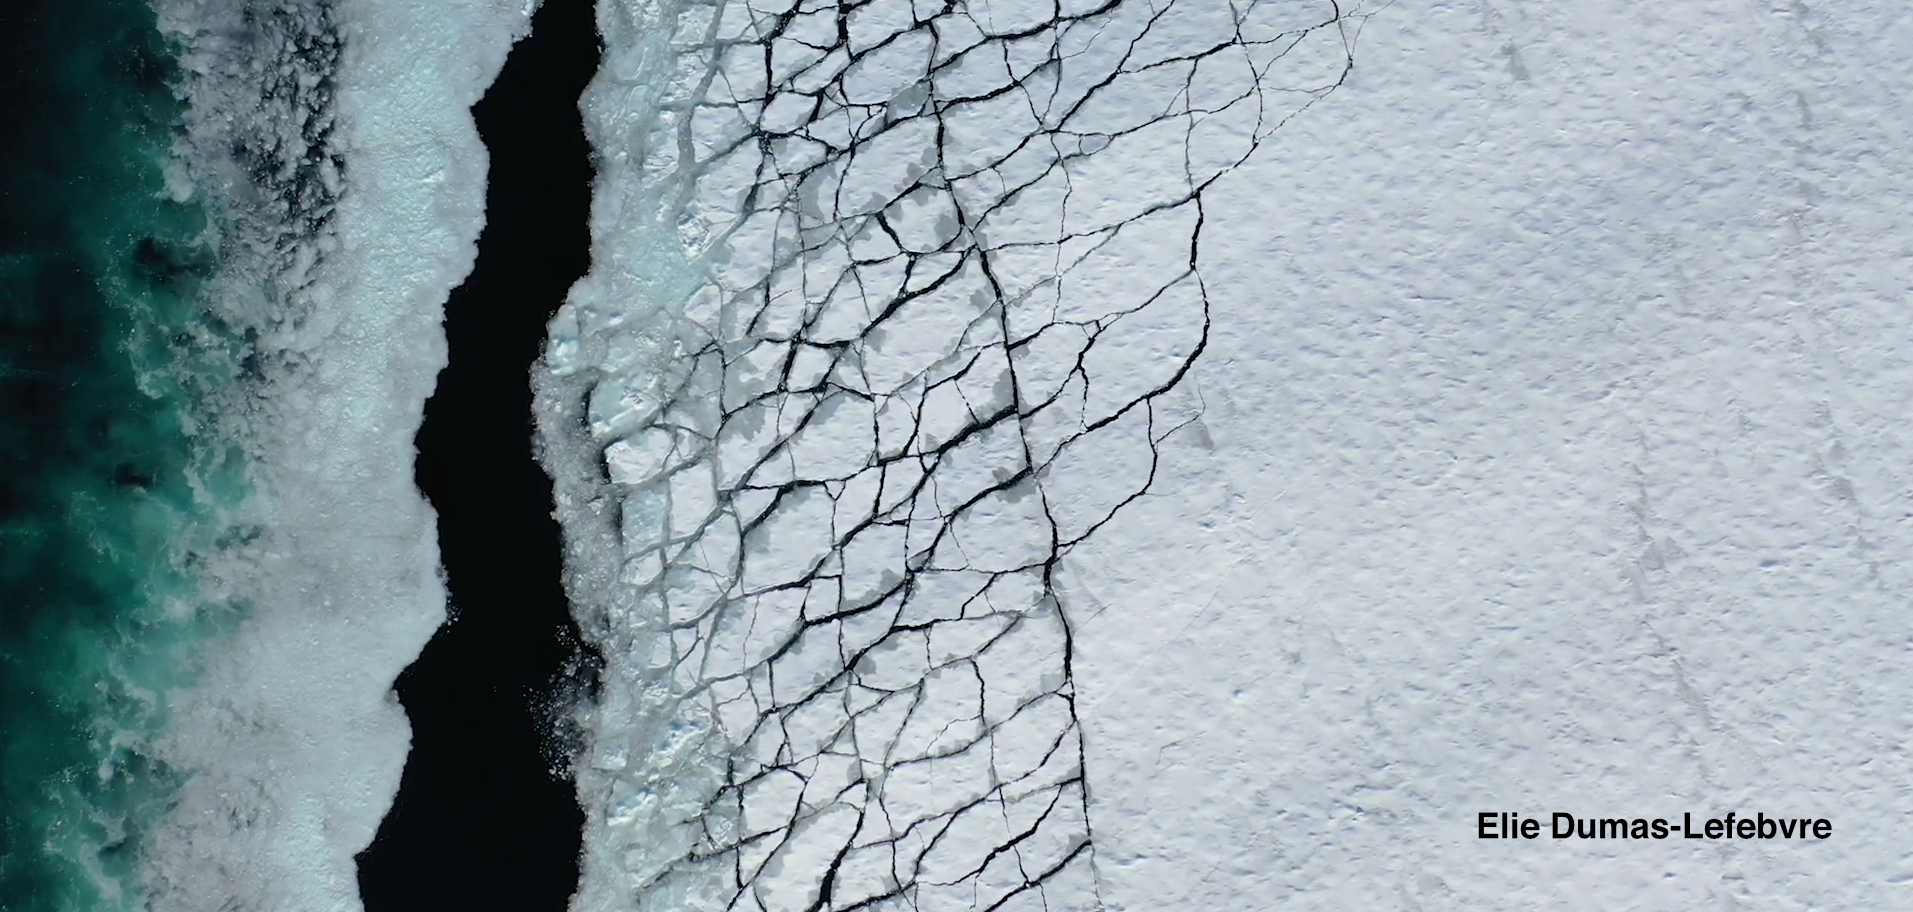
\includegraphics[width=.9\textwidth]{./figures/Lefebvre.png}}{./videos/lefebvre_video.mp4}
  \end{figure}
\end{frame}


\begin{frame}{Le dispositif expérimental}
\begin{figure}
  \centering
  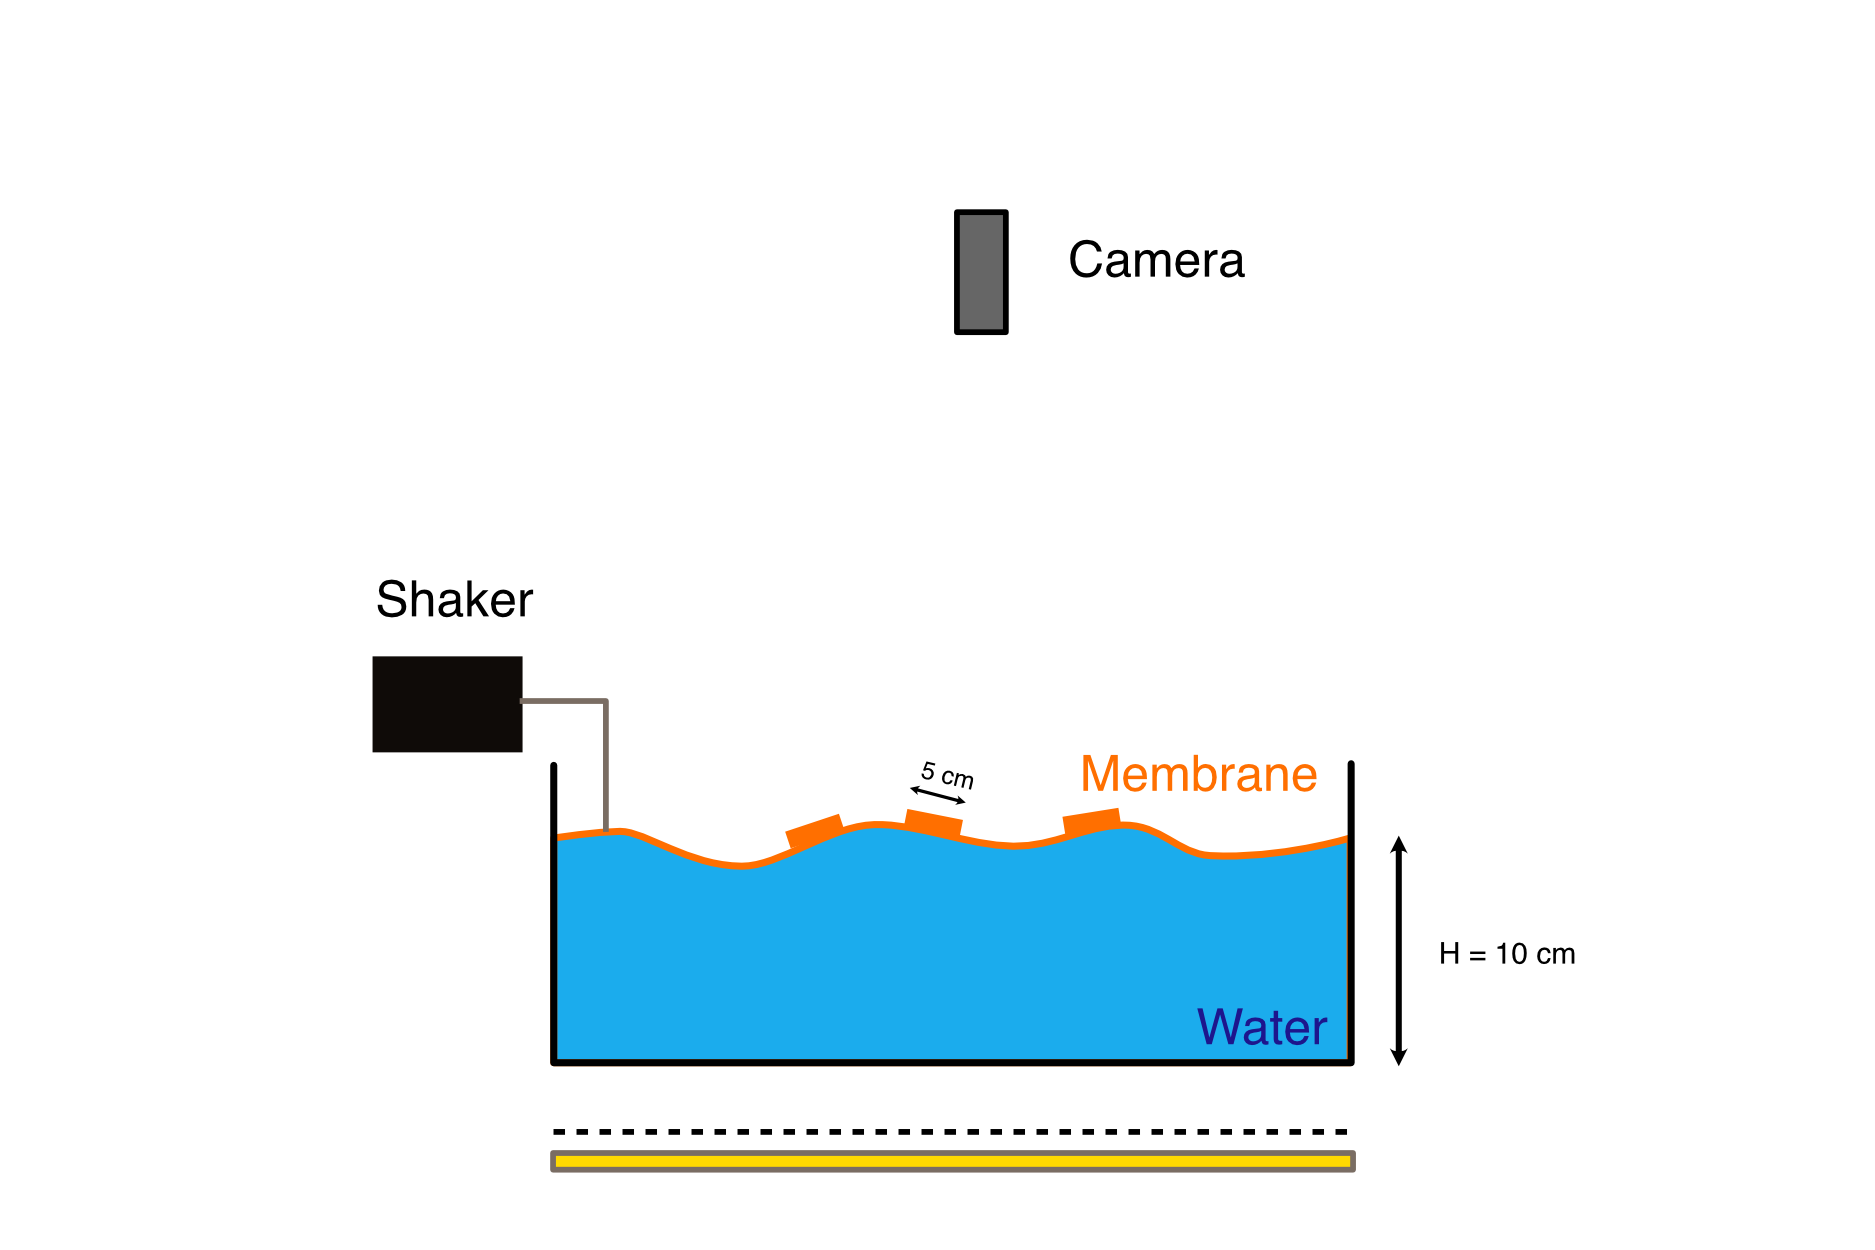
\includegraphics[width=.8\textwidth]{./figures/Setup.png}
\end{figure}
\end{frame}

\begin{frame}{Technique expérimentale}
\begin{figure}
  \centering
  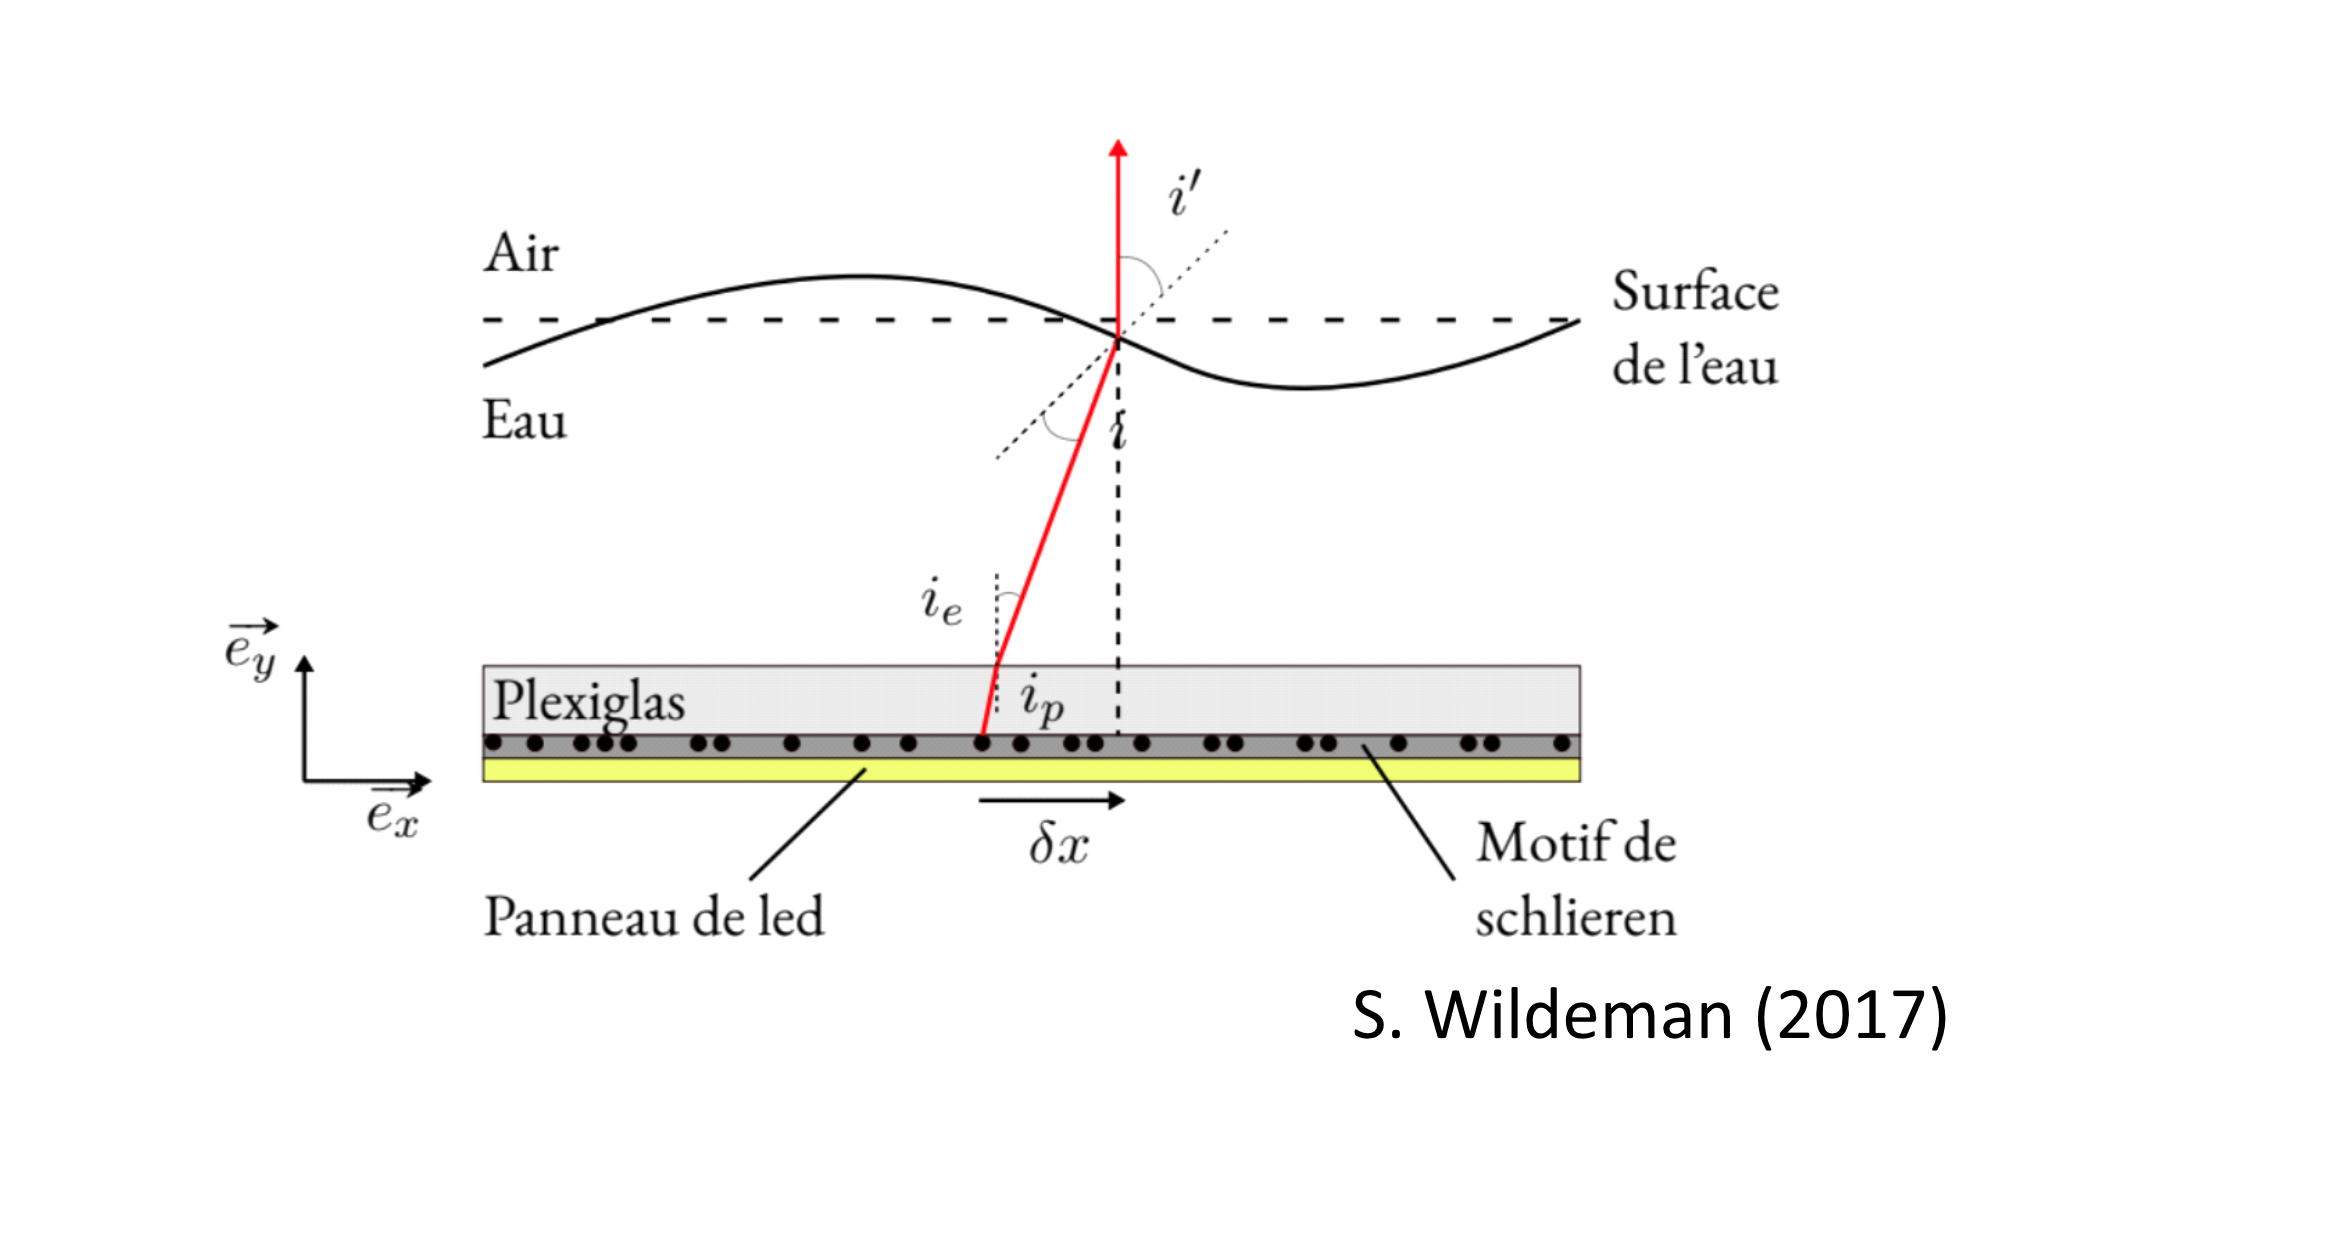
\includegraphics[width=.9\textwidth]{./figures/fcd.png}
\end{figure}
\end{frame}

\begin{frame}{Mesure du champ de déformation (f = 150 Hz)}
\begin{figure}
  \centering
  \movie{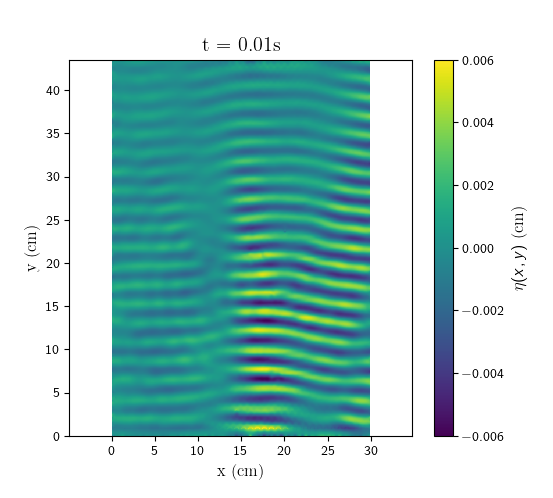
\includegraphics[width=.6\textwidth]{./figures/Champ_deformation_mean_n0.png}}{./videos/Movie_mean_demod_test_deformation.avi}
\end{figure}

\end{frame}

\begin{frame}{Relation de Dispersion}
\noindent \textbf{Navier Stokes equation:}
\begin{equation}
  \rho \dfrac{\partial v}{\partial t}  + \rho (v \cdot \nabla )v = -\nabla P + \eta \Delta v + \rho g
\end{equation}

\noindent \textbf{Équation de Föppl-Von Karman  (mécanique des plaques):}
\begin{equation}
  \underbrace{D\Delta^2\eta}_{\rm Énergie~ de~ pliage} - \underbrace{e\dfrac{\partial }{\partial x_\beta}\left(\sigma_{\alpha,~\beta}\dfrac{\partial \eta}{\partial x_{\alpha}}\right)}_{\rm Étirement}=\underbrace{F}_{\rm Forces~ extérieures}.
\end{equation}

\begin{itemize}
  \item Rigidité à la flexion $D=\dfrac{Ee^3}{12(1-\nu^2)}$
  \item Module d'Young $E$: $\rm E(glace) = 9\cdot 10^9~Pa$, $E(membrane) \approx 7\cdot 10^6\rm~ Pa.$;
  \item $\nu$ coefficient de Poisson  $\nu\approx 0.25$;
  \item $\sigma$ contrainte.
\end{itemize}

\end{frame}

\begin{frame}{Relation de dispersion }
\noindent \textbf{Navier Stokes:}
\begin{equation}
  \rho \dfrac{\partial v}{\partial t}  + \rho (v \cdot \nabla )v = -\nabla P + \eta \Delta v + \rho g
\end{equation}
\noindent \textbf{Föppl-Von Karman:}
\begin{equation}
  D\Delta^2\eta - e\dfrac{\partial }{\partial x_\beta}\left(\sigma_{\alpha,~\beta}\dfrac{\partial \eta}{\partial x_{\alpha}}\right) = F.
\end{equation}
\begin{center}
\noindent Grande longueur d'onde par rapport au déplacement vertical: $\eta_0 \ll \lambda.$\\
\end{center}
\noindent \textbf{fonction d'onde:}
\begin{equation}
  \Phi(x,z,t) = \phi(z){\rm e}^{i(\omega t -kx)}.
\end{equation}
\noindent \textbf{Relation de dispersion des ondes hydro-élastiques:}
\begin{ombredef}
  \begin{defi}
    \begin{equation}
      \omega^2 = gk + \dfrac{T}{\rho}k^3 + \dfrac{D}{\rho}k^5.
    \end{equation}  
  \end{defi}
\end{ombredef}
\end{frame}

\begin{frame}{Mesure de la relation de dispersion (Thèse Lucie Domino)}

\begin{figure}
  \centering
  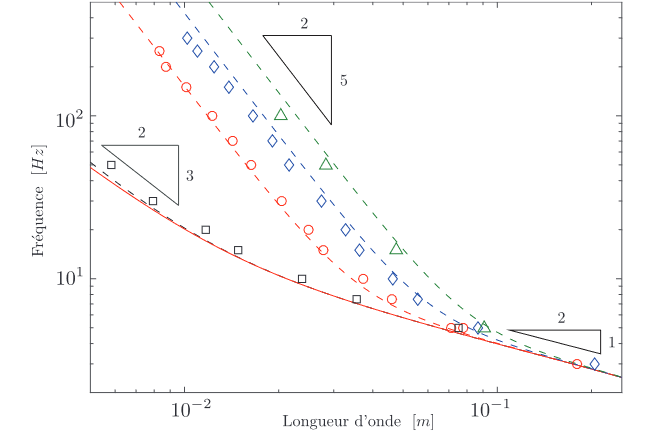
\includegraphics[width = .5\textwidth]{./figures/Lucie_Domino.png}
\end{figure}
\centering
\begin{ombretheo}
  \begin{theo}
    \textbf{Pente 1/2:} Régime gravitaire grande longueur d'onde $\lambda$.\\
    \textbf{Pente 3/2:} Régime de tension pour un $\lambda$ intermédiaire.\\
    \textbf{Pente 5/2:} Régime de flexion aux petits $\lambda$.  
  \end{theo}
\end{ombretheo}
Plus l'épaisseur de la membrane est grande plus on entre dans le régime élastique
\end{frame}


\begin{frame}{Environment Hétérogène  (1 disque $d=5~\rm cm$, $f=150~\rm Hz$, $A = 600~\rm mV$ ) }
\begin{figure}
  \centering
  \movie{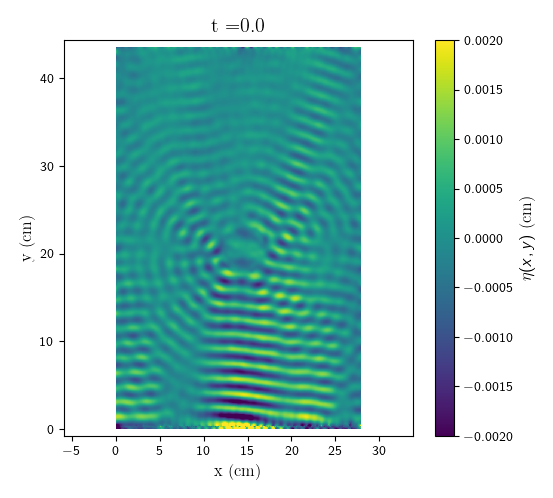
\includegraphics[width=.6\textwidth]{./figures/Champ_deformation_mean_n0_1disk_f150Hz_A600mV.png}}{./videos/Movie_mean_demod_deformation_1disk.avi}
\end{figure}
\end{frame}


\begin{frame}{Environment Hétérogène (2 disques, $d=5~\rm cm$, $f=150~\rm Hz$, $A = 600~\rm mV$ ) }

\begin{figure}
  \centering
  \movie{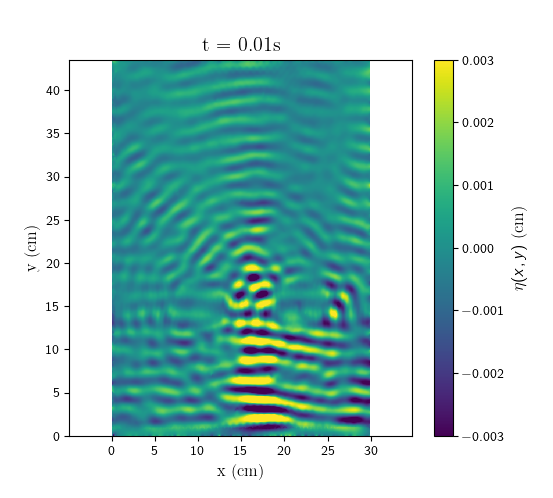
\includegraphics[width=.6\textwidth]{./figures/Champ_deformation_mean_n0_2disk_f150Hz_A600mV.png}}{./videos/Movie_mean_demod_test_deformation_2disks.avi}
\end{figure}

\end{frame}


\begin{frame}{Environment Hétérogène (3 disques, $d=5~\rm cm$, $f=150~\rm Hz$, $A = 600~\rm mV$ ) }
\begin{figure}
  \centering
  \movie{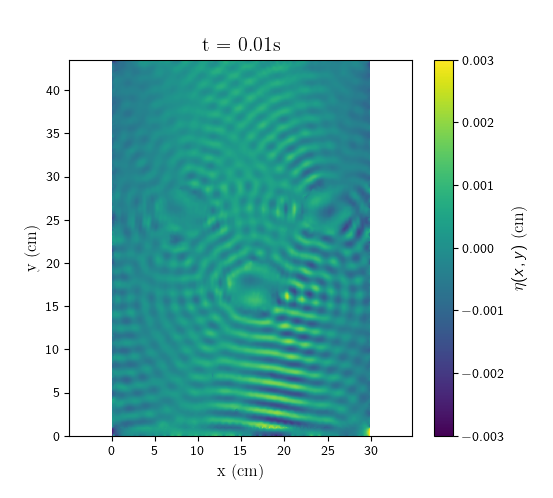
\includegraphics[width=.6\textwidth]{./figures/Champ_deformation_mean_n0_3disks_f150Hz_A600mV.png}}{./videos/Movie_mean_demod_test_deformation_3disks.avi}
\end{figure}
\end{frame}


% \begin{frame}{Breaking the Ice - Bapstiste Internship}
% \end{frame}

% \begin{frame}{Measurements of fragments'sizes}
% \end{frame}

 
\end{document}


% \begin{frame}{Sommaire}
%     \tableofcontents
% \end{frame}

% \begin{frame}
%     \section{Rappels généraux sur la tension de surface} 
% \end{frame}

% \input{Introduction.tex}

% \input{Generation_vorticite.tex}

% \begin{frame}
%     \section{Partie 2 : Propulsion par effet Marangoni}
% \end{frame}

% \input{Propulsion_bateaux.tex}

% \begin{frame}
%     \section{Conclusion}
% \end{frame}

% \begin{frame}{Conclusion}
%     \begin{minipage}{7cm}
%         \textbf{Partie 1: Génération de vorticité}\\[0.1cm]
%         \hspace{-1cm}\begin{figure}
%             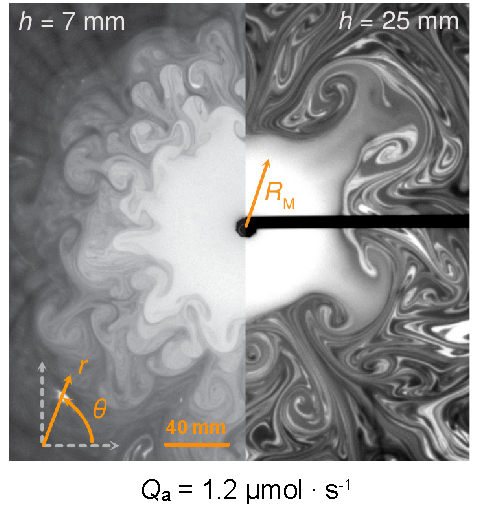
\includegraphics[width=.8\textwidth]{./figures/Marangoni_conclusion.pdf}
%         \end{figure}   
%     \end{minipage}
%     \begin{minipage}{6.7 cm}
%         \textbf{Partie 2: Propulsion des bateaux}
%         \begin{figure}
%             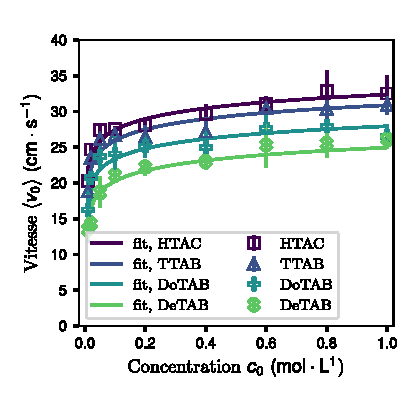
\includegraphics[width=1\textwidth]{./figures/Bateaux/Bateau_v0_final.pdf}
%         \end{figure}
%     \end{minipage}
% \end{frame}

% \begin{frame}{Merci pour votre attention}
%         \begin{figure}
%           \movie{\includegraphics[width=.8\textwidth]{./figures/51130819085_7cc767c08d_k.jpg}}{./videos/video-carangoni-test-2.mov}
%         \end{figure}
% \end{frame}

% % \begin{frame}{Remerciements}
% %     \begin{figure}
% %         \centering
% %         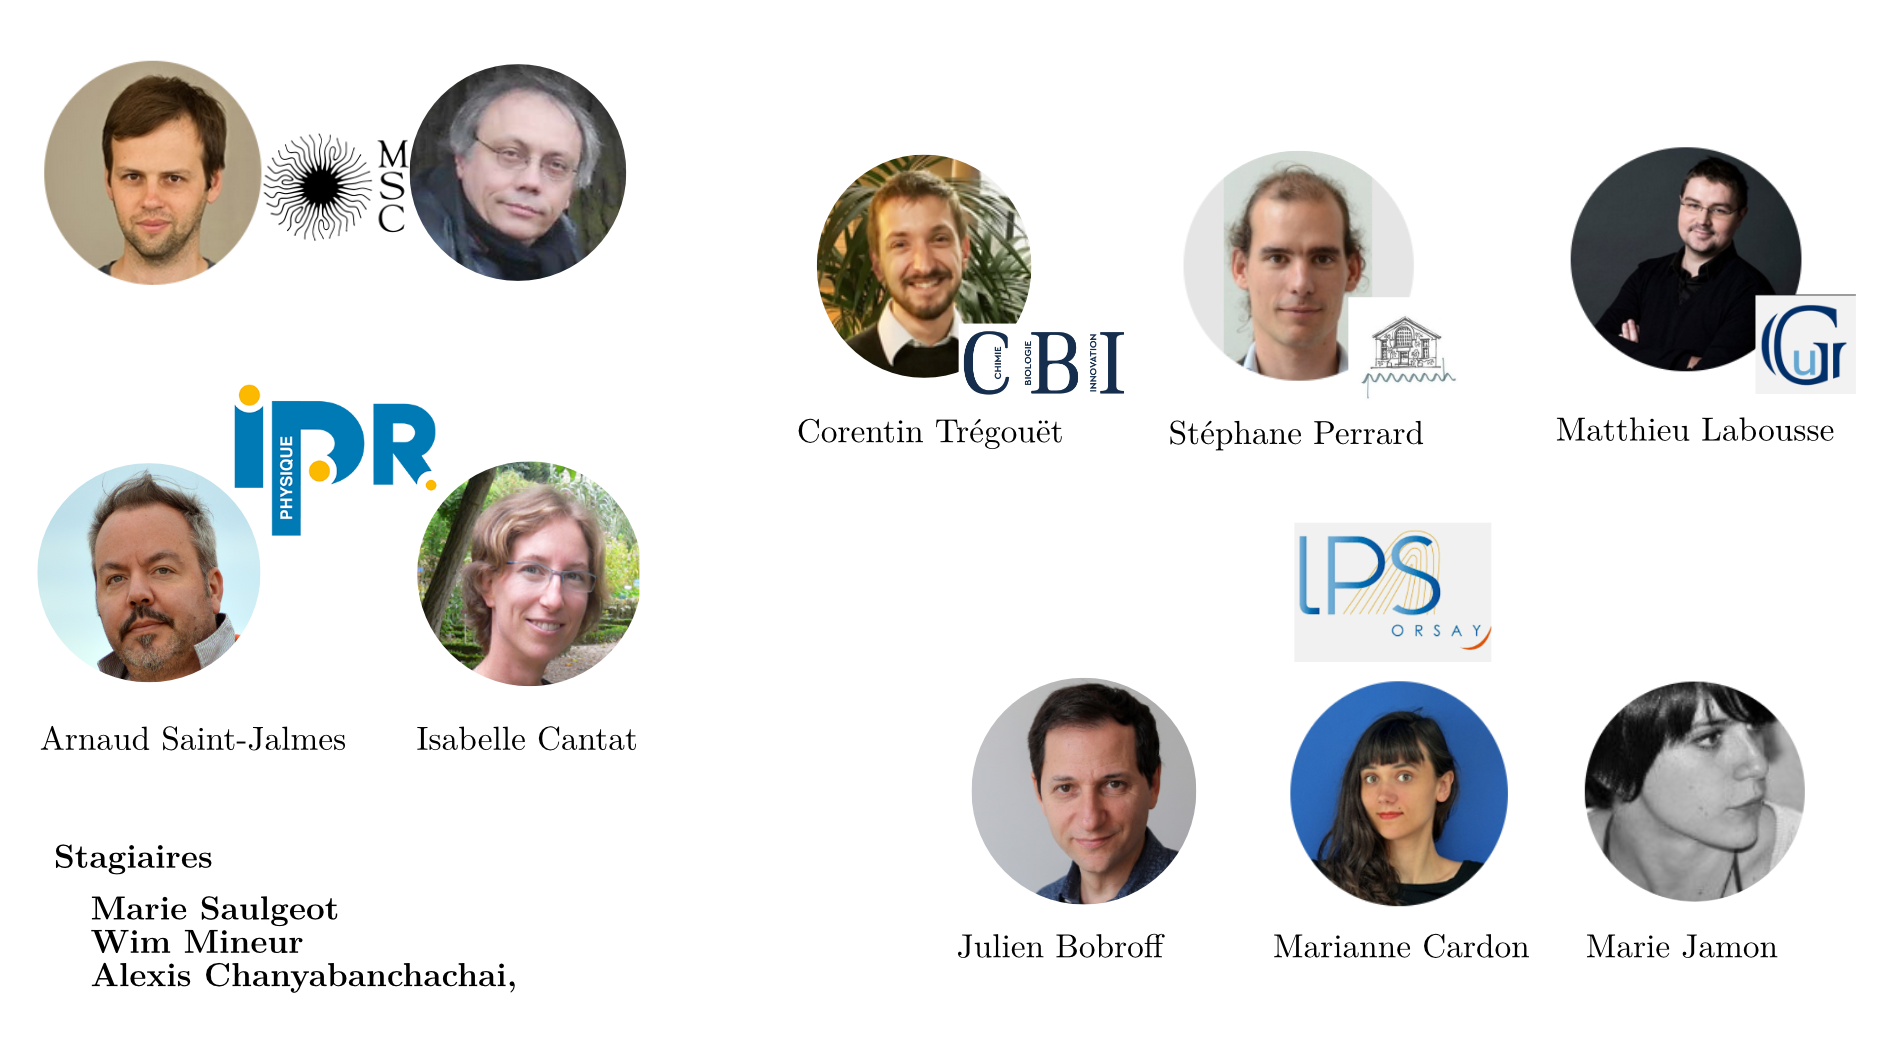
\includegraphics[scale=.8]{./figures/Collaborations.png}
% %     \end{figure}
% % \end{frame}


% \begin{frame}
%     \section*{Annexes}
% \end{frame}

% \input{Annexe.tex}

% \begin{frame}
%     \bibliographystyle{apalike}%apalike}%abbrv}
%     \bibliography{MaTheseBiblio.bib}
% \end{frame}

% \end{document}

% %%% Local Variables:
% %%% mode: latex
% %%% TeX-master: t
% %%% End:

